\documentclass[a4paper,10pt,twocolumn]{article}
%\usepackage{xeCJK}
%\setCJKmainfont{SimSun}
\usepackage{CJKutf8}
\usepackage{cite}
\usepackage{listings}
\usepackage[T1]{fontenc}
\usepackage{amsmath}
\usepackage{amssymb}
\usepackage{graphicx}
\usepackage[]{circuitikz}
\setlength{\oddsidemargin}{0in}
\setlength{\topmargin}{-.8in}
\setlength{\textheight}{9.7in} \setlength{\textwidth}{6.5in}
\usepackage{color,hyperref}
\definecolor{darkblue}{rgb}{0.0,0.0,0.3}
\hypersetup{colorlinks,breaklinks,
            linkcolor=darkblue,urlcolor=darkblue,
            anchorcolor=darkblue,citecolor=darkblue}
\providecommand*\url[1]{\href{#1}{#1}}
\renewcommand*\url[1]{\href{#1}{\texttt{#1}}}

\newcommand{\bm}[1]{\boldsymbol{#1}}
\newcommand{\bh}[1]{\boldsymbol{\hat{#1}}}
\newcommand{\bt}[1]{\boldsymbol{\tilde{#1}}}
\newcommand{\bbar}[1]{\boldsymbol{\bar{#1}}}
\newcommand{\mbf}[1]{\ensuremath{\mathbf{#1}}}
\newcommand{\ode}[2]{\ensuremath{\frac{\mathrm{d} #1}{\mathrm{d} #2}}}
\newcommand{\odet}[2]{\ensuremath{\tfrac{\mathrm{d} #1}{\mathrm{d} #2}}}
\newcommand{\oden}[3]{\ensuremath{\frac{\mathrm{d}^#3 #1}{\mathrm{d} #2^#3}}}
\newcommand{\pde}[2]{\ensuremath{\frac{\partial #1}{\partial #2}}}
\newcommand{\pdet}[2]{\ensuremath{\tfrac{\partial #1}{\partial #2}}}
\newcommand{\pden}[3]{\ensuremath{\frac{\partial^{#3} #1}{\partial
      #2^{#3}}}}
\newcommand{\sub}[1]{\ensuremath{_{\rm{#1}}}}
\newcommand{\arriba}[1]{\ensuremath{^{\rm{#1}}}}
%
\newcommand{\N}{\ensuremath{\mathbb{N}}}
\newcommand{\R}{\ensuremath{\mathbb{R}}}
\newcommand{\C}{\ensuremath{\mathbb{C}}}
\newcommand{\ee}[1]{\ensuremath{\mathrm{e}^{#1}}}
\newcommand{\hdos}{\ensuremath{\mathrm{H}_2}}
\newcommand{\COdos}{\ensuremath{\mathrm{CO}_2}}
\newcommand{\ATP}{\ensuremath{\mathrm{ATP}}}

\newcommand{\dt}{\ensuremath{\mathrm{d}t}}
\newcommand{\dtau}{\ensuremath{\mathrm{d}\tau}}
\newcommand{\DV}{\ensuremath{\Delta V}}
\DeclareMathOperator{\Li}{\mathcal {L}^{-1}}
\DeclareMathOperator{\Lin}{\mathcal {L}^{-1}}
\DeclareMathOperator{\sinc}{\text{sinc}}
\DeclareMathOperator{\sign}{\mathrm{sign}}
\newtheorem{remark}{Remark}
%\usepackage[utf8x]{inputenc}
%%
\title{围棋 \\ The Game of Go\\ \small Modeling Complex Systems\\ DMKM}
\author{Carlos López Roa\\ \href{mailto:me@mr3m.me}{me@mr3m.me}}
\date{\today}
\pdfinfo{%
  /Title    ()
  /Author   (CLR)
  /Creator  ()
  /Producer ()
  /Subject  ()
  /Keywords ()
}
\begin{document}
\begin{CJK*}{UTF8}{gbsn}
\maketitle
\lstset{
basicstyle=\tiny,
numbers=left,
numberstyle=\tiny,
numbersep=5pt, 
showspaces=false,
showstringspaces=false,
showtabs=False,
frame=false,
%tabsize=.5,
keywordstyle=\bfseries\color{green!40!black},          % keyword style
 commentstyle=\itshape\color{purple!40!black},       % comment style
  stringstyle=\color{gray},
basicstyle=\ttfamily}

%%% Content
\begin{abstract}
Go is an ancient, simple, rather complex board game. It is now posed as the frontier in game theory for artificial intelligence applications. In this work we develop a MAS\footnote{Multi Agent Systems} approach of the game of Go, the theory and implementation is explained and some results are proven. A video demo of the implementation is available on this \href{https://youtu.be/Wvm0ZgCsm1E}{link}. Also the Source Code can be found on \href{https://github.com/mr3m/GameOfGo}{GitHub}
\end{abstract}

%\tableofcontents

\section{Introduction}
The game of Go, also known as {Wéiqí: 围棋} in Chinese, which means literally \emph{surround game}, is a two-player board game in which the aim is to surround more territory that the opponent \cite{Kunkle2002}.

It was originated in ancient China more than 2,500 years ago (figure \ref{l1}). It was considered one of the four essential arts\footnote{The four arts ({siyi: 四艺}): To play the guqin, a stringed instrument ({Qín:  琴}), the strategy game of Go ({Qí:  棋}), Chinese calligraphy ({Shu:  书}), Chinese painting ({Huà:  画}) } of a cultured Chinese scholar.

\begin{figure}[!ht]
\begin{center}
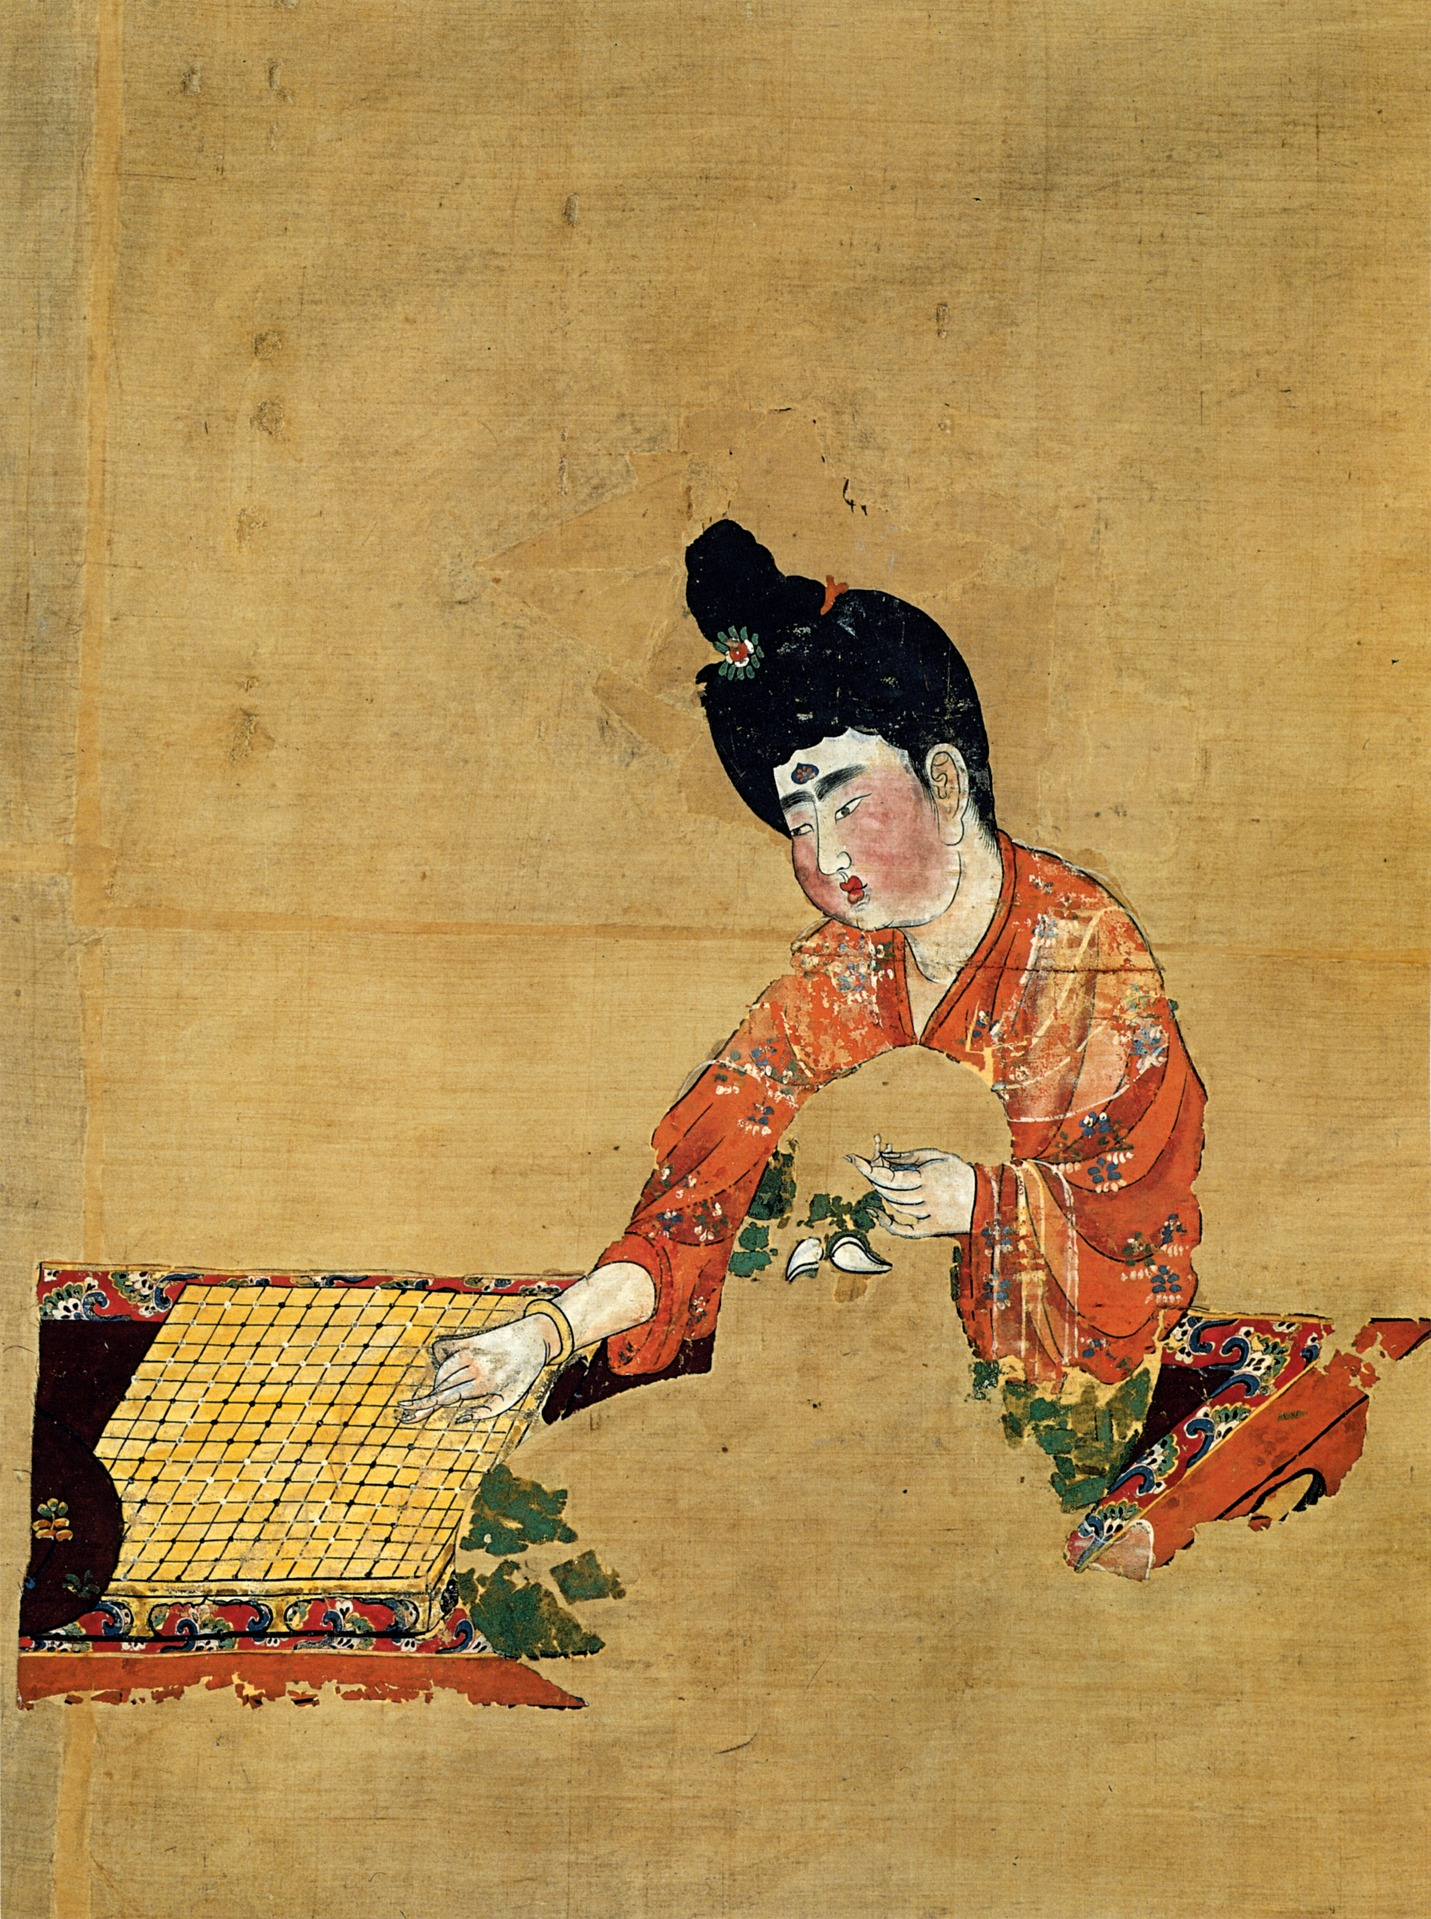
\includegraphics[width=4cm]{Astana.jpg}
\caption{\footnotesize{Woman Playing Go (Tang Dynasty c. 744), discovered at the Astana Graves}\label{l1}}
\end{center}
\end{figure}

Despite it's relative simple rules, the relative complexity of Go with respect to Western chess is far more superior ($10^{761}$ compared to $10^{120}$ possible games).

Precisely because of this great complexity is that, different from chess which was \emph{conquered} by IBM's \textsc{Deep blue} in 1996 agains't world's Grand Master \textsc{Gary Kaspárov}, no equivalent conquest has been achieved by computer go until recent victory of Google's \textsc{Alpha Go} agains't \textsc{Fan Hui} the European Go Champion \cite{Silver2016a}. 

In this study we took a multiagent system approach to the problem of computer Go, first, a description of the implementation is made, after some tests were carried out and described at the end some conclusions and future work are drawn.

%\subsection{State of the art}

\subsection{Game Mechanics}
The two players alternately place black and white playing pieces, called \emph{stones}, on the vacant places of a board with a 19×19 grid of lines\footnote{Fast games can be played in 9x9 or 13x13 boards}. 

Each stone is said to have 4 \emph{liberties} ({Qì:  气})  when the four orthogonal-adjacent points are empty, this stone loses each of it's liberties whenever a stone is placed in this points. If the recently placed stone is of the opposite color, then the liberty is just lost, however, if the recently placed stone is of the same color, the individual liberty is lost and a \emph{group} liberty is created, composed of the sum of the liberties of these two stones. Generalizing the previous principle, one can form huge groups of stones of the same color, which have a collective liberty. The particular form of this groups is essential part of the strategy of the game. 

Once placed on the board, stones may not be moved, but stones may be removed from the board if captured. A stone (or group of stones) it's captured by the opponent when all the liberties are suppressed.

 An enclosed liberty (or liberties) is called an \emph{eye}\footnote{see figure \ref{f1}} (眼), and a group of stones with at least two separate eyes is said to be unconditionally \emph{alive}. Such groups cannot be captured, even if surrounded. \emph{Dead} stones are stones that are surrounded and in groups with poor shape (one or no eyes), and thus cannot resist eventual capture.

\begin{figure}[!ht]
\begin{center}
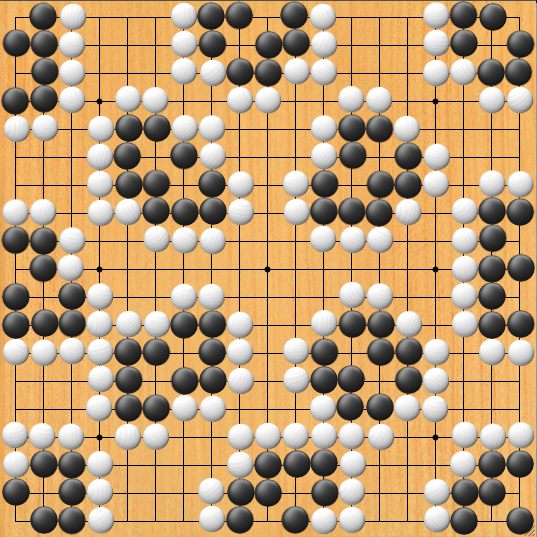
\includegraphics[width=5.5cm]{eyes.png}
\caption{\footnotesize All the smallest groups with two eyes by blacks, enclosed by whites without being able to capture the groups \label{f1}}
\end{center}
\end{figure}

There are only two rules in Go, namely: 

\begin{enumerate}
\item \textbf{The rule of Liberty}: Every stone remaining on the board must have at least one liberty.
\item \textbf{The ko rule (劫)}: The stones on the board must never repeat a previous position of stones
\end{enumerate}

Remark that by rule 1, suicide moves are forbidden, that is jumping into an eye of the opponent contained in a at-least-two-eye-group; if the group is a one-eye-group then this move is allowed. Also please note that to blocks one eye, though permitted is by no means desired, since it can turn alive groups into dead ones. Also as a common consensus, blacks play first.   

The two players place stones alternately until they reach a point at which neither player wishes to make another move. When a game concludes, the territory is counted along with captured stones to determine the winner. 

\section{Implementation}
A box world was set up in NetLogo, to represent the board game, that is, with no periodicity in the edges.  

In this world, two computers play Go agains't each other. Though, the computer players are composed of the collective decision of the stones placed in the board, that is, using the distributed artificial intelligence approach of multiagent systems. 

The stones were modeled using reactive agents, the environment is a 19x19 closed two dimensional grid, all agents share the same organization, the interaction between each other happens when they share a liberty. Also agents of the same color connected through their liberties form undirected links between each other.  The goal, is the same as the game, to occupy the most territory.  The game ends when both agent types pass consecutively. 

\subsection{Making a move}
A general overview of the game dynamics can be seen in the flow diagram \ref{d1}

\begin{figure}[!ht]
\begin{center}
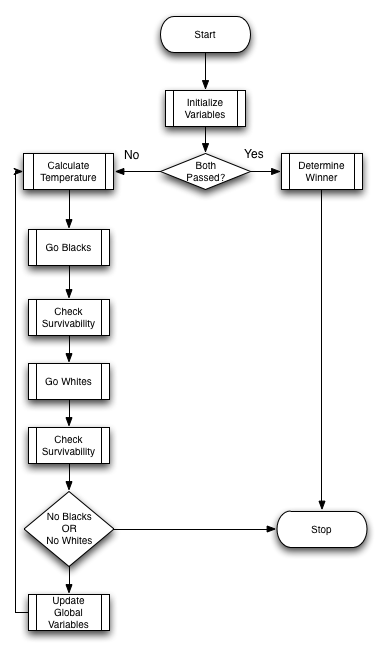
\includegraphics[width=7cm]{df.png}
\caption{\footnotesize {Flow diagram of the main components of the program.} First we initialize the variables. A if condition governs the flow, which is the condition to end the game.  \label{d1}}
\end{center}
\end{figure}

Each turtle has four internal variables: The number of liberties, the number of captured stones, the liberties of the group in which they are in, and a boolean variable related to the exploration of groups. 
 
Each patch in the environment has a temperature associated, which is composed of the number of stones surrounding this patch, that is a measure of liberty of the patch. 

To make a move, we follow the flow described in diagram \ref{d2}

\begin{figure}[!ht]
\begin{center}
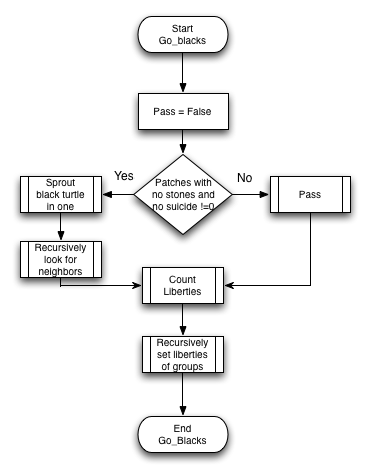
\includegraphics[width=7cm]{go_blacks.png}
\caption{\footnotesize Flow to play blacks. To play whites is simmetrical. A IF statement looks for free patches, if found a black turtles is sprout and related with it's neighbours recursively, if not then blacks pass. Then this stone is assigned their liberties, and the groups get the liberties recalculated.\label{d2}}
\end{center}
\end{figure}

To calculate the liberties of one turtles is just to subtract the number of stones in the neighboring spaces from the number of neighboring spaces\footnote{corner stones get between 3 and 2 instead of 4 neighboring spaces}, the group liberty is defined as the sum of the individual liberties. If both the individual liberty and the group one are equal to zero, then the stone (group) dies. 

The discovery of the group of one stones is done by asking each stone to name it's neighbors recursively, when all neighbors have been named, then we assign an undirected link between this stone and all the named neighbors. This due to the transitivity: If $A$ is neighbor of $B$ and $B$ is neighbor of $C$ then $A$ is neighbor of $C$.

Thing to note, is that because of the condition to pass, then it's not possible to commit suicide or to block owns eyes. 

\section{Results}

In general, the computer plays well, that is, with no illegal plays, and the game is always stopped by both players passing their turns (figure \ref{r1})

\begin{figure}[!ht]
\begin{center}
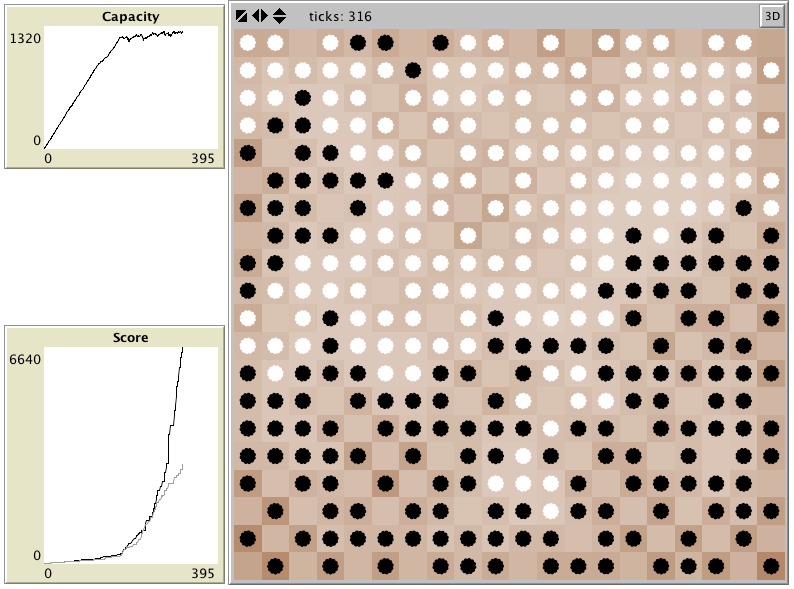
\includegraphics[width=8cm]{game1.png}
\caption{\footnotesize Random final result of a game between the two computer players. We observe a final state with big at-leat-two-eyed structures and no further plays to make. Also we can observe the score with respect to time, and we see the capturing contribution to the score leading to blacks victory. Also the capacity shows that the map saturated in the mid game. \label{r1}}
\end{center}
\end{figure}

To prove the \emph{fairness} of the game, we ran 2,000 games on different sizes of the board, (9x9, 13x13 \& 19x19) to look at the winner and scores in each case with similar results, results show in figures \ref{rr1} and \ref{rr2}.

\begin{figure}[!ht]
\begin{center}
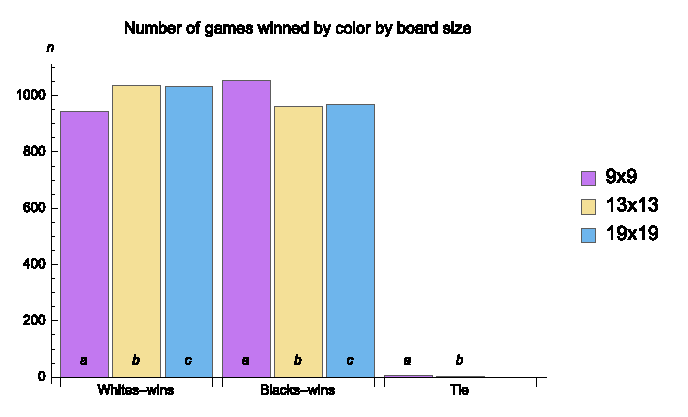
\includegraphics[width=8cm]{r1.eps}
\caption{\footnotesize We can see that across board sizes the the proportion is mantained. \label{rr1}}
\end{center}
\end{figure}

The empirical probabilities to win in a 19x19 board size are: Whites:$51.55\%$ and Blacks $48.45\%$. That is, empirically there's no preference for any player over the other. 


\begin{figure}[!ht]
\begin{center}
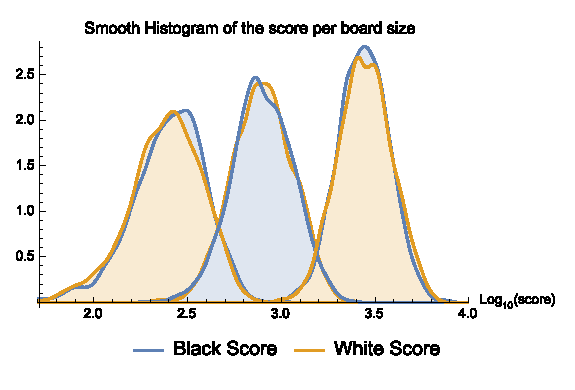
\includegraphics[width=8cm]{r2.eps}
\caption{\footnotesize Here we see the distribution of the Logarithm of the score, the lowest score corresponds to 9x9 the middle one to 13x13 and the greatest to 19x19 board size respectively. We can see that in each case the distribution is quite similar, that is, there's no particularity on the scores of one player over the other.  \label{rr2}}
\end{center}
\end{figure}

\section{Conclusions}
We can draw the following conclusions. 

\begin{itemize}
\item Gathering the fairly simple rules of go we were able to construct a multi agent system based model of the game. 
\item The model can replicate behavior that a single player may exhibit such as, resigning, non suicide, capture and control. 
\item More complex behavior of groups of stones are well modeled such as, group assembling and eye formation and conservation. 
\item The game is well modeled since no illegal moves are done, and each time the game ends\footnote{no infinite loops}. 
\item The empirical proportion of games won by player and the distribution of the score, does not vary significantly neither with the board size, nor with the color of the player. 
\item The game is fair 
\end{itemize}

\section{Future Work}

So far we have developed a fair model of the game of Go, the main strategy to make a move is a random choice of all the legal moves. We can develop more complex strategies on top of the existing model, for example by using the temperature measure. 

Also, since we can test two different computer strategies in the same game, we can prove the superiority of one strategy on top of another. 
\bibliography{/Users/Poincare/Dropbox/Tex/library.bib}
\bibliographystyle{siam}
\newpage
\onecolumn
\appendix

\section{Appendix: Source Code}
\begin{lstlisting}[language=]
globals [
  global-temperature        ;Shown as capacity of the world
  num-blackss               ;number of black stones plus captured white stones
  num-whitess               ;number of white stones plus captured black stones
  scenario-phase            
  global-score-blacks       ;max of individual stored captured blacks
  global-score-whites       ;max of individual stored captured whites
  blacks-pass               ;Boolean, has blacks passed?
  whites-pass               ;Boolean, has whites passed?
  winner                    ;String, Who is the winner?
  ]

breed [blacks]    ;Two breeds
breed [whites]
undirected-link-breed [teams team] ;Undirected links

patches-own [temperature]   ;Liberty of the patch

blacks-own [      ;Internal variables of stones
  libertynot      ;The liberty of the stone
  score-blacks    ;Internal score of blacks captured
  libertygroup    ;The liberty of the group
  explored?       ;Bolean, is he explored in recursive search
]

whites-own [
  libertynot 
  score-whites
  libertygroup
  explored?
]

to setup   ;Set variables
  clear-all
  set-default-shape blacks "flower"
  set-default-shape whites "flower"
  ask patches [ set pcolor gray ]
  set winner nobody
  set global-temperature 0
  ask blacks [set score-blacks 0]
  ask whites [set score-whites 0]
  set blacks-pass false
  set whites-pass false
  seed-blackss-randomly  ;Initiallize two stones 
  seed-whitess-randomly
  ask patches [calc-temperature]
  set global-temperature (mean [temperature] of patches)
  update-display
  reset-ticks
end

to seed-blackss-randomly  ;It was necessary to use a observer procedure
     go_blacks			;to call a turtle procedure
end

to seed-whitess-randomly
     go_whites
end

to go  ;Turtle procedure, To go
  ifelse not blacks-pass or  not whites-pass 
  [ ;Main IF, has both passed sucesively?
   ask patches [calc-temperature] ;Update patch color
   diffuse temperature .5
   go_blacks                         
   ask whites [check-survivability]
   go_whites
   ask blacks [check-survivability]
   if (num-whitess = 0 or num-blackss = 0 ) [stop] 
   ;update global variables
   set global-temperature (sum [temperature] of patches) 
   set global-score-blacks (max [score-blacks] of blacks ) 
   set global-score-whites (max [score-whites] of whites )
   ask blacks [set score-blacks max [score-blacks] of blacks]
   ask whites [set score-whites max [score-whites] of whites]
   update-display
   tick
  ]
  [ if num-blackss > num-whitess  ;Determine winner
    [set winner "Blacks"]
    if num-blackss < num-whitess
    [set winner "Whites"]
    if num-blackss = num-whitess
    [set winner "Tie"]
    output-print (word winner "-wins,"  num-blackss ","  num-whitess ) 
    ;Print Winner
    stop]
end

to experiment  ; Experimentation procedure, to keep creating games
    if winner != nobody [setup]
    go
end

to set-as-blacks  
  set color black 
  set size 0.6
  set explored? false 
  create-links-with turtles-on neighbors4 with [any? blacks-here] 
  ;make group with neighbors
  loop    ;Recursively make group with the neighbors of neighbors 
  [ let start one-of blacks with [not explored?]  
    if start = nobody [stop]
    ask start [explore]
    ask blacks [ set explored? false ]
    stop
  ]
end

to set-as-whites  
  set color white
  set size 0.6
  set explored? false 
  create-links-with turtles-on neighbors4 with [any? whites-here]
  loop
  [ let start one-of whites with [not explored?]
    if start = nobody [stop]
    ask start [explore]
    ask whites [ set explored? false ]
    stop
  ]
end

to explore ;Recursively set explored
  if explored? [stop]
  set explored? true
  ask link-neighbors [explore]
  if breed = blacks [
  create-links-with other blacks with [explored?]]
  if breed = whites [
  create-links-with other whites with [explored?]]
end


to check-survivability   ;Kill if no liberties 
  if libertynot = 0 and libertygroup = 0
  [
  if (breed = whites)  
    [ask whites [set score-whites (score-whites + count(link-neighbors) + 1) ]
    ;Give the score to the other player
     ask link-neighbors [die] ;Ask all members of the group to die
     die] ;Before dying
  if (breed = blacks)
    [ask blacks [set score-blacks (score-blacks + count(link-neighbors) + 1) ]
      ask link-neighbors [die]
      die]
  ]
end

to go_blacks
  set blacks-pass false  
  ifelse count (patches with [not any? whites-here  and not any?  blacks-here  
  and (count (turtles-on neighbors4 with [any? whites-here]) < count(neighbors4))
  and (count (turtles-on neighbors4 with [any? blacks-here]) < count(neighbors4))
    ]) != 0 ;Are there any patches to put stones?
  [
  ask n-of 1 patches with [not any? whites-here  and not any?  blacks-here
  and (count (turtles-on neighbors4 with [any? whites-here]) < count(neighbors4))
  and (count (turtles-on neighbors4 with [any? blacks-here]) < count(neighbors4))
    ] ;Pick one
     [ sprout-blacks 1 [set-as-blacks] ] ; Create one turtle there
  ]
  [set blacks-pass true
  ]
   ask blacks [set libertynot count(neighbors4) - count(turtles-on neighbors4) 
;Set individual liberty
   set libertygroup (sum [libertynot] of link-neighbors + libertynot)] 

;Set group liberty
end

to go_whites
  set whites-pass false
  ifelse count (patches with [not any? blacks-here and not any? whites-here
  and (count (turtles-on neighbors4 with [any? blacks-here]) < count(neighbors4))
  and (count (turtles-on neighbors4 with [any? whites-here]) < count(neighbors4))
    ]) != 0
    [
  ask n-of 1 patches with [not any? blacks-here and not any? whites-here
  and (count (turtles-on neighbors4 with [any? blacks-here]) < count(neighbors4))
  and (count (turtles-on neighbors4 with [any? whites-here]) < count(neighbors4))
    ]
     [ sprout-whites 1 [set-as-whites] ]
    ]
   [set whites-pass true]
   ask whites [set libertynot count(neighbors4) - count(turtles-on neighbors4)
   set libertygroup (sum [libertynot] of link-neighbors + libertynot)]
end


to calc-temperature  
  set temperature (count(turtles-on neighbors4)) ;The liberty of a patch
end

to paint-blacks    ;Manual input of stones
  if mouse-down?
  [
    ask patch mouse-xcor mouse-ycor [
      ifelse not any? blacks-here
      [
        if paint-blacks-as = "add black"
          [sprout-blacks 1 [set-as-blacks]]
        if paint-blacks-as = "add white"
          [sprout-whites 1 [set-as-whites]]
      ]
      [
        if paint-blacks-as = "remove"
          [ask blacks-here [die]]
      ]
      display  
    ]
  ]
end

to update-display  ;Plotting options
  ifelse (show-temp-map? = true)
    [ ask patches [set pcolor scale-color brown temperature -7 7] ]  
    [ ask patches [set pcolor grey] ]

  ifelse (show-blacks? = true)
    [ ask blacks [set hidden? false] ]
    [ ask blacks [set hidden? true] ]
    
  ifelse (show-connections? = true)
   [ ask links [set hidden? false] ]
    [ ask links [set hidden? true] ]
end
\end{lstlisting}



\end{CJK*}
\end{document}